% Standalone document
\documentclass[notes.tex]{subfiles}
\begin{document}
%%%%%%%%%%%%%%%%%%%%%%%%%%%%%%%%%%%%%%%%%%%%%%%%%%%%%%%
%%%%%%%%%%%%%%%%%%%%%%%%%%%%%%%%%%%%%%%%%%%%%%%%%%%%%%%
\chapter{Supersymmetric dark matter}
\label{chap:dm}
%%%%%%%%%%%%%%%%%%%%%%%%%%%%%%%%%%%%%%%%%%%%%%%%%%%%%%%
%%%%%%%%%%%%%%%%%%%%%%%%%%%%%%%%%%%%%%%%%%%%%%%%%%%%%%%

We have a standard model also for cosmology, the Lambda Cold Dark Matter model ($\Lambda$CDM). This models the observed universe on three main ingredients: the known Standard Model matter (dominantly the baryonic matter of the atoms, radiation and neutrinos), dark energy ($\Lambda$) and cold dark matter (CDM), where the cold signifies that this ingredient is non-relativistic. In this chapter we will look closer at candidates for dark matter (DM) in supersymmetric models.



%%%%%%%%%%%%%%%%%
\section{Evidence for dark matter}
%%%%%%%%%%%%%%%%%
The idea of dark matter goes back quite a long way. Today we have evidence for the existence of dark matter through several effects where we observe its gravitational influence on ordinary matter. We list the evidence below:
\begin{enumerate}[1)]
\item Kinematics  (Zwicky 1933~\cite{Zwicky:1933gu}): The motion of galaxies (velocity dispersion) cannot be explained by the visible matter. This has also been observed on the scales of galaxies in their rotation curves (Rubin 1970~\cite{Rubin:1970zz}).
\item Gravitational lensing (Tyson 1996~\cite{Fischer:1996eb}). First observed in galactic clusters. Clusters show evidence of lensing not explained by luminous matter.  Dark matter dynamics (non-interacting) are demonstrated by the Bullet cluster (Clowe 2006~\cite{Clowe:2006eq}). 
\item Large scale structures (clusters, superclusters, filaments and voids): The structures observed in the 2dFGRS (2-degree Field Galaxy Redshift survey~Colles 2001~\cite{Hawkins:2002sg}) and the SDSS (Sloan Digital Sky Survey~Tegmark 2004~\cite{Abazajian:2004it}) imply a relative matter density of $\Omega_m \equiv \frac{\rho_m}{\rho_c} \simeq  0.29$ where $\rho_c = 1.05\cdot 10^{-5}h^2$\,GeV/cm$^3$ is the critical energy density for a flat universe.\footnote{$h$ is defined through the Hubble constant $H_0$ as $H_0=100 h$\,km/Mpc/s.} They also imply that the majority of DM must be {\bf cold} (non-relativistic), because warm DM would suppress clustering.
\item Big-Bang Nucleosynthesis (BBN): The formation of light elements in the period $t = 1-1000$\,s after the Big Bang. Measurements of Early Universe abundance of light elements, mainly D and He, points to a baryonic matter density of $\Omega_b \approx 0.04$. This gives $\Omega_{\text{leftover}}=\Omega_{\text{DM}} \approx 0.25$.
\item Supernovae (Riess 1998~\cite{Riess:1998cb} and Perlmutter 1999~\cite{Perlmutter:1999jt}): Measurements of type Ia supernovae (SNe Ia) were used as standard candles to show an accelerated expansion of the Universe. This fixes $\Omega_\Lambda-\Omega_m \simeq k$ where $\Omega_\Lambda$ is the energy density of dark energy/cosmological constant.
\item Cosmic Microwave Background (CMB) (Penzias \& Wilson 1965~\cite{Penzias:1965wn}): The temperature variation of the CMB over the sky of the order of $0.0002$\,K is sensitive to all cosmological parameters, and gives $\Omega_\Lambda +\Omega_m \simeq k$, where $k$ is some constant.
\end{enumerate}

The evidence above can be used to constrain the $\Lambda$CDM concordance model of cosmology, which has just a handful of ingredients such as baryonic and dark matter, radiation (photons) and dark energy. In Fig.~\ref{fig:LambdaCDMfit} we show the effects of the SNe, CMB and large scale structure data (BAO) on this model in the plane of matter density $\Omega_\text{m}$ and dark energy density $\Omega_\Lambda$.

%%%
\begin{figure}[h!] 
\includegraphics[width=0.5\textwidth]{figures/DMfit.eps} 
\caption{Limits from different observational sources on the dark energy density, $\Omega_\Lambda$, compared to the total mass density in the universe, $\Omega_m$.}
\label{fig:LambdaCDMfit}
\end{figure}
%%%

A maximum likelihood fit to a selected subset of the measurements by the Planck Collaboration~\cite{Ade:2013zuv} gives the parameters for the model shown in Table~\ref{tab:LambdaCDM}. This means that the non-baryonic matter constitutes some 85\% of the matter in the Universe, and that its relative energy density is quite well determined, at the percent level.

\begin{table}[h!]
\begin{tabular}{l |c| c| c| c| c} 
\hline
Parameter & $\Omega_\Lambda$ & $\Omega_\text{m} h^2$ & $\Omega_b h^2$ & $H_0$\,[km/Mpc/s] & $t_0$\,[Gy]\\\hline
Value & $0.685^{+0.018}_{-0.016}$& $0.1426\pm 0.0025$ & $0.02205 \pm 0.00028$ & $67.3\pm 1.2$ & $13.817 \pm 0.048$ \\
\end{tabular}
\caption{Measured values for cosmological parameters~\cite{Ade:2013zuv}.}\label{tab:LambdaCDM}
\end{table}



%%%%%%%%%%%%
\section{WIMP magic}
%%%%%%%%%%%
The very existence of a stable Weakly\footnote{Weak as in electro-weak, meaning on the same scale as the weak force.} Interacting Massive Particle (WIMP) $\chi$ automatically gives an additional component to the total energy density of the Universe. WIMPs are found in a number of theories, for example the lightest neutralino of the MSSM, the lightest Kaluza-Klein particle of a theory with extra dimensions or an inert (no vev) Higgs boson. 

This is due to the in equilibrium {\bf thermal production} of the WIMP through the process $SM\ SM \to \chi \chi$, where $SM$ are some Standard Model particles, and the reverse annihilation process $\chi \chi \to SM\ SM$, in the early hot Universe ($T\gg m_\chi$). As the temperature decreases to $T< m_\chi$ and there is not enough energy in an average collision for the production of $\chi$ to occur, only the reverse process can take place, and the comoving density\footnote{Taking the expansion of the universe into account by looking at the number of particles in a volume expanding at the same rate.} falls with the temperature of the Universe. 

The WIMPs then experience what is called a {\bf chemical decoupling}, or loss of chemical equilibrium, due to the expansion of the Universe. This is when the WIMPs become so dilute, because of the expansion, that they in effect no longer interact inelastically, and this roughly happens when the expansion rate becomes larger than the rate of annihilation. The WIMPs then get a constant (comoving) density, we say that they experience a {\bf freeze-out} at this temperature $T_c$. With weak-scale masses and couplings the freeze-out happens at $T_c \approx 0.05 m_{\chi}$, however, this is before or at the same time as {\bf kinetic decoupling} where the WIMPs effectively lose elastic interactions with the other matter, meaning that $\chi$ freezes-out with non-relativistic velocities and become cold dark matter.

The exact time (temperature) of freeze-out is controlled by the annihilation cross section of $\chi$, larger cross sections keep chemical equilibrium for longer, in turn resulting in lower dark matter relic abundance. This abundance, in number density, can be found from the Boltzmann equation
\begin{equation}
\frac{dn_\chi}{dt} = -3H n_\chi - \langle \sigma v \rangle (n_{\chi}^2 - n_{\chi}^{eq}{}^2),
\end{equation}
where $n_{\chi}^{eq}$ and $n_{\chi}$ are the chemical equilibrium and actual comoving number densities, $H$ is Hubble's constant for the expansion rate, and $\langle \sigma v\rangle$ the velocity averaged annihilation cross section for $\chi\chi \to SM\ SM$. Solutions to this equation for increasing  $\langle \sigma v\rangle$ are shown in Fig.~\ref{fig:freeze_out}.

%%%
\begin{figure}[h!]
\begin{center}
\includegraphics[width=0.9\textwidth]{figures/freezeout.eps} 
\caption{Illustration of the freeze-out of the comoving number density of a WIMP as a function of time, where the black line represents a model without chemical decoupling, and the dotted lines represent different freeze out temperatures for different velocity averaged annihilation cross sections.}
\label{fig:freeze_out}
\end{center}
\end{figure}
%%%

In practice one must also often take into account co-annihilation with other particles with mass within $10\% - 20\%$ of the $\chi$, and numerical codes such as {\tt DarkSUSY}~\cite{Gondolo:2004sc} or {\tt MicrOMEGAs}~\cite{Belanger:2001fz,Belanger:2004yn} are typically used to solve the Boltzmann equation. For weak scale particles a rough approximation to the resulting dark matter density is 
\[\Omega_\chi h^2 = 0.1 \times \frac{3\times 10^{-26}\,{\rm cm}^3 {\rm s}^{-1}}{\langle \sigma v \rangle},\]
and since the annihilation cross section can be shown to be
\begin{equation}
\langle \sigma v \rangle \approx \frac{\alpha_{weak}^2}{m_{weak}^2} \approx 10^{-25}\,{\rm cm}^3 {\rm s}^{-1},
\end{equation}
the predicted dark matter density is
\[\Omega_\chi h^2 \approx 0.1 \times \left(\frac{g_{weak}}{g_\chi}\right)^4\left(\frac{m_\chi}{m_{weak}}\right)^2.\]
When compared to the values in Table~\ref{tab:LambdaCDM} this is called the {\bf WIMP-miracle} since it supplies just about the correct missing energy density for the WIMP as long as it has a weak scale mass and a weak scale coupling to the Standard Model. The strong sensitivity of the predicted dark matter density to both the mass and the coupling, and the precisely measured experimental value, means that the WIMP scenario is very predictive and testable.

For a more detailed discussion of the WIMP miracle, see the standard cosmology book by Kolb and Turner~\cite{Kolb:1990vq}.



%%%%%%%%%%%%%%%%%%%%%%%%%%
\section{Dark matter candidates in supersymmetry}
%%%%%%%%%%%%%%%%%%%%%%%%%%
With R-parity conservation in place we have seen that the LSP is stable and any neutral LSP can then in principle constitute all or part of the dark matter. Without R-parity only super-weakly coupling particles like gravitinos and axinos are candidates. Below we briefly discuss the various possibilities.


%%%
\subsection{Neutralino}
%%%
As soon as you have a stable neutralino LSP, you usually get into trouble trying to explain why there is so little dark matter. For example, the standard mSUGRA bino-like $\tilde\chi^0_1$ scenario prefers LSP masses around 100 GeV or lower not to overproduce dark matter. Due to current lower bounds on the $\tilde{\chi}^0_1$ mass and the measured Higgs mass this tends to be difficult to realise in practise. 
This scenario with a low mass bino-like neutralino is often called the {\bf bulk region} scenario, which can be seen in Fig.~\ref{NeuDM} in the lower left corner.  

%%%
\begin{figure}[h!]
\begin{center}
\includegraphics[width=\textwidth]{figures/NeutralinoDM.eps} 
\caption{Generic illustration of the allowed neutralino dark matter regions (puke green) in the $(m_0,m_{1/2})$-plane for mSUGRA. Except for the low $m_0$ and $m_{1/2}$ regions the area outside of the allowed green region gives too much dark matter. The dashed line shows the Higgs mass limit which pushes towards larger values of $m_{1/2}$, while the dotted line represents the limit from the anomalous magnetic moment of the muon.\label{NeuDM}}
\end{center}
\end{figure}
%%%

Alternatives to the bulk region scenario use co-annihilation or resonant annihilation to increase $\langle \sigma v \rangle$ and thus decrease the dark matter density. The {\bf stau-coannihilation region}, where $\tilde{\tau}_1 \tilde{\chi}^0_1 \to SM\, SM$ is an efficient annihilation process reducing the dark matter density, exists for $m_{\tilde{\tau}_1} - m_{\tilde{\chi}^0_1}\leq 10$\,GeV. This makes the scenario difficult to discover at collider experiments due to the production of soft (low-energy) taus. In mSUGRA the stau-coannihilation region can be found for small $m_0$, and is shown as the lower strip in Fig.~\ref{NeuDM} which follows the lower theoretical bound (brown) where the stau becomes the LSP. Outside of mSUGRA similar regions can also be found for smuons and selectrons, with large  mass degeneracy between the slepton and the LSP.

The {\bf stop-coannihilation region}, where $\tilde{t}_1 \tilde{\chi}^0_1 \to SM\, SM$ is efficient typically has $m_{\tilde{t}_1} - m_{\tilde{\chi}^0_1}\leq 25$\,GeV. In mSUGRA this exists for large values of $|A_0|$, small $m_0$ and $m_{1/2}$. Again, this is difficult to discover because of the soft decay products of the stop.

The {\bf Higgs funnel region} is found for $2 m_{\tilde{\chi}^0_1} \simeq m_{A,H}$ and large $\tan \beta$, where the neutralino has resonant annihilation through a heavy Higgs boson. For mSUGRA, this is shown in Figure \ref{NeuDM} as the two diagonal structures roughly in the middle of the plot, rising as a funnel upwards.

The {\bf chargino-coannihilation} region can be found when we have higgsino or wino LSPs, where a chargino is automatically degenerate with the LSP resulting in a lower dark matter density typically below experimental bounds. In mSUGRA this region is called the  {\bf focus point region}, and is found for large $m_0$ and low $\mu$, leading to so-called split-SUSY, as the sfermion masses need to be pressed up quite a bit, and there is a large mass difference between gauginos and sfermions. The focus point region can be seen in Fig.~\ref{NeuDM} following the upper theoretical bound where EWSB breaks down.


%%%
\subsection{Sneutrinos}
%%%
The left handed sneutrino $\tilde{\nu}_L$ is happily excluded as a potential dark matter candidate due to the large cross section for  $\tilde{\nu}_L q \to \tilde{\nu}_L q$ via $Z$-exchange.\footnote{For the neutralinos this problem only exists for a higgsino $\tilde{\chi}^0_1$ LSP, as the wino and bino do not couple to the $Z$.} The large cross means that it should already have been seen by direct detection experiments, see Sec~\ref{sec:DD}. It is also problematic to get $m_{\tilde{\nu}_L}<m_{\tilde{l}_L}$ due to hyperfine-splitting. However, the right-handed sneutrino $\tilde{\nu}_R$ couples very weakly and is still a viable candidate. This would necessitate adding right-handed neutrinos and sneutrino superfields to the MSSM.


%%%
\subsection{Gravitino}
%%%
The {\bf gravitino} is the massive spin-3/2 supersymmetric partner of the graviton in models with supergravity. With only gravitational strength interactions, the gravitino is {\it not} a WIMP as it is never in chemical equilibrium. If it is the LSP it can be created from the decays of the next-to-lightest supersymmetric particle (NLSP), giving, in R-parity conserving scenarios,
\[\Omega_{\tilde{G}} = \frac{m_{\tilde{G}}}{m_\text{NLSP}}\Omega_\text{NLSP}.\]
However, these scenarios are problematic because the NLSP is long-lived due to the extreamly weak interaction and creates potential trouble in BBN by injecting energy that changes the production of light elements. 

Alternatively, the gravitino can be created in non-thermal production processes in the period of reheating after inflation. One potential process $gg \to \tilde{g}\tilde{G} $ is shown in Fig.~\ref{gravterm}. The reverse process $\tilde{g}\tilde{G} \to gg$ is not efficient as the density of gravitinos is never high enough given the small cross section. This type of dark matter creation process is often called {\bf freeze-in}. For the gravitino this gives a new magic formula:
\begin{equation}
\Omega_{\tilde{G}}h^2 \approx 0.5 \cdot \left(\frac{T_R}{10^{10}\,{\rm GeV}}\right)\left(\frac{100\,{\rm GeV}}{m_{\tilde{G}}}\right)\left(\frac{m_{\tilde{g}}}{1\,{\rm TeV}}\right)^2,
\end{equation}
where $T_R$ is the unknown and very weakly constrained reheating temperature. This production mechanism is also valid for models with R-parity violation. There the small gravitino coupling $\propto \frac{1}{M_P}$ makes the gravitinos very long-lived, with lifetimes longer than the age of the Universe, but not absolutely stable because of the R-parity violating operators. 
%One can also imagine an axino scenario, that would work just like the gravitino.


%%%
\begin{figure}[h!]
\begin{center}
\includegraphics{figures/gravterm.eps} 
\caption{One possible diagram for the non-thermal production of gravitinos from the scattering of gluons.\label{gravterm}}
\end{center}
\end{figure}
%%%


%%%
\subsection{Others}
%%%
One could even imagine colour charged supersymmetric particles as dark matter, in particular the gluino, which, if stable, after hadronisation with Standard Model quarks and/or gluons would form so-called {\bf R-hadrons}. These have very strict limits from searches, but these limits are somewhat obfuscated by complications in modelling R-hadron scattering.



%%%%%%%%%%%%%
\section{Direct detection}
\label{sec:DD}
%%%%%%%%%%%%%
In addition to the direct production of dark matter at colliders and the corresponding searches for missing energy, there are two other main ways to search for dark matter, direct and indirect detection. Here we briefly discuss {\bf direct detection}.

Direct detection seeks to make weak and thus rare dark matter interactions with standard model matter visible by very low background searches in large volumes, using local galactic halo dark matter interacting with ordinary matter on Earth. The feasibility of direct detection  is very dependent on the $\chi$ scattering cross section on nucleons (quarks), which can in principle be calculated in a given model,\footnote{However, while the quark--dark matter cross section is relatively easy to calculate, the fact that the quark is bound in a nucleon, and the nucleon bound to a nucleus makes this more difficult in practice, involving also estimates from nuclear physics.} but also on the dark matter halo density distribution and velocity distribution, which have large uncertainties. 

The rate of interaction between dark matter and a particular type of nucleons in a sample can be expressed in the differential scattering rate with respect to the recoil energy $E_r$ of a scattered nucleon with mass $M$ as
\begin{equation}
\frac{dN}{dE_r} = \frac{\sigma \rho_{DM}}{2\mu^2 m_\chi}|F(q)|^2\int_{v_{min}}^{v_{esc}} \frac{f(\vec v)}{v}d^3v,
\label{eq:DD_rate}
\end{equation}
where $\sigma$ is the dark matter scattering cross section off the nucleus in question, $\rho_{DM}$ is the dark matter halo density at Earth, $\mu=m_\chi M/(m_\chi+M)$ is the dark matter and nucleus reduced mass, $F(q)$ is a nuclear form factor dependent on the scattering momentum transfer $q=\sqrt{2ME_r}$ and the nucleon type, $f(\vec v)$ is the velocity distribution of the dark matter in the halo, $v_{min}=\sqrt{ME_r/2\mu^2}$ is the minimal velocity that gives a recoil energy $E_r$ and $v_{esc}$ is the escape velocity from the halo.

In general direct detection relies heavily on suppressing Standard Model backgrounds which would be the overwhelmingly dominant cause of observed recoils. This is done by moving the experiments deep under ground where they are shielded from cosmic rays, and by specifically shielding the detector samples against local radioactivity. Beyond this, there are  two main tactics followed in order to try to directly detect dark matter:
\begin{itemize}
\item Suppress (almost) all backgrounds and monitor as large a volume as possible. This used in experiments such as XENON, PANDAS and CDMS.
\item Look for an annular modulation in the event rate -- due to the Earth's movement in the galactic rest frame and thus in the dark matter halo, changing the velocity integral in Eq.~(\ref{eq:DD_rate}) -- to observe a small dark matter signal on top of a constant background, such as used in the DAMA and CoGeNT experiments.
\end{itemize}

Figure~\ref{fig:DD_exclusion} shows results from the current most important direct detection experiments as limits on the dark matter--nucleon cross section as a function of dark matter mass. Observe that while DAMA claims a detection (closed regions), these are already excluded by many other experiments. For reference, a neutralino WIMP could reasonably be expected to have a scattering cross section in the range $10^{-45}-10^{-50}$ cm$^2$ for masses in the range 100--1000 GeV~\cite{GAMBIT:2017zdo}. The dashed yellow line shows what is called the {\bf neutrino floor}. This is the cross section that can be reached before the experiments would be saturated with recoils due to neutrinos scattering off the experiment sample. Going below the neutrino floor would need new experimental techniques, fundamentally, the direction of the particle creating the recoil would need to be reconstructed.

%%%
\begin{figure}[h!]
\begin{center}
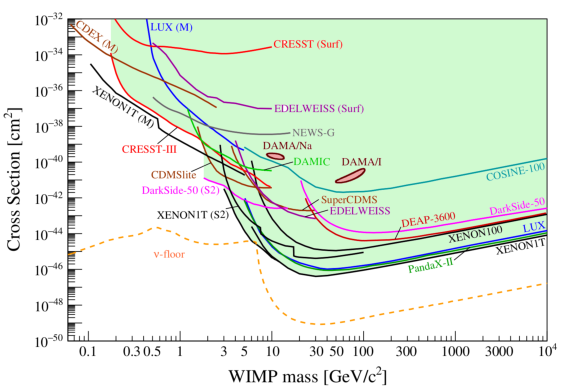
\includegraphics[width=\textwidth]{figures/APPEC_si_current_limits} 
\caption{Plot of different exclusion and detection results for direct detection of dark matter in the WIMP mass versus WIMP--nucleon cross section plane~\cite{Billard:2764484}. The dashed yellow line shows the neutrino floor. }
\label{fig:DD_exclusion}
\end{center}
\end{figure}
%%%


%%%%%%%%%%%%%
\section{Indirect detection}
%%%%%%%%%%%%%
In {\bf indirect detection} we look for the annihilation, $\chi\chi\to SM\, SM$, or decay products of dark matter in multiple final (messenger) states in cosmic rays. The viable search channels must be stable Standard Model particles, so that they can reach the Earth (or satellites in orbit). The messengers should also have as low backgrounds from ordinary astrophysical processes as possible, this makes searches with electrons and protons extra challenging. The remaining candidates are photons, neutrinos, positrons, antiprotons and antideuterons.\footnote{Potentially, even heavier antinuclei than antideuterons could be used, but they would be even rarer.} We now discuss the properties of each of these in a little more detail.

%
\subsubsection{Photons} 
These can either come from direct production processes such as the annihilation channels $\chi\chi \to \gamma \gamma, Z\gamma$, which is relatively easy to detect because the spectrum is a sharp line at exactly the mass of the dark matter, or they could be $\gamma$ from bremsstrahlung or pion decays in the annihilation decay products, which creates a broad spectrum. This is harder to detect because of the large background of bog-standard astrophysical photons, but is expected to make up the majority of photons from dark matter. Photons from dark matter have the advantage that they point to the source, so we can focus our searches on areas in our galaxy or nearby galaxies with large $\rho_{DM}$, where annihilation or decay is more probable, and thus reducing potential backgrounds relative to the signal. We can also look for photons that are extragalactic in origin, but then we have to account for the red-shifting of the spectrum.

Dark matter annihilating in our own galaxy into photons should result in a differential flux at Earth in terms of energy $E$ and solid angle $\Omega$ given by
\begin{equation}
\frac{d\Phi}{dE d\Omega} = \frac{1}{8\pi m_\chi^2}\frac{dN_\gamma}{dE}\langle \sigma v \rangle \int_{\text{l.o.s.}} \rho^2_{DM}(l) dl,
\end{equation}
where $N_\gamma (E)$ gives the number of photons with energy $E$ in a single annihilation event and the integral is over the dark matter density in the line of sight. We see that the flux depends on the square of the dark matter  density since annihilation requires two  particles to be present. For decaying dark matter the corresponding expression is proportional to $\rho_{DM}$.

There have been some indications of an excess of photons above expected backgrounds from the galactic centre (a.k.a.\ the Hooperon~\cite{Hooper:2010mq}), however, no unambiguous dark matter signal has been confirmed. Current limits from the Fermi-LAT experiment seems to rule out most possible models for  a dark matter  explanation for this excess, and, more importantly, sets a cross section limit for dark matter annihilation close, and for some masses beyond, to the canonical limit of
\[\langle\sigma v\rangle = 3\times 10^{-26}\,{\rm cm}^{3}{\rm s}^{-1},\]
which would give the correct dark matter density, see Fig.~\ref{fig:FERMI}.\footnote{Keep in mind though, that the velocity distribution of any dark matter today would not be the same as during freeze-out at a much higher temperature, so the cross section numbers are not exactly translatable.} This limit is some of the strongest evidence today against WIMP dark glitter.

%%%
\begin{figure}[t!]
\begin{center}
\includegraphics[width=0.9\textwidth]{figures/FERMI_dSph_bb.eps} 
\caption[Fermi-LAT results]{Results from Fermi-LAT indirect gamma-ray searches in the $\chi\chi\to b\bar b$ channel. Grey line shows limit from Milky Way halo search, black line from Milky Way dwarf spheroidal galaxy search with six years of data~\cite{Ackermann:2015zua}. \label{fig:FERMI}}
\end{center}
\end{figure}
%%%

%
\subsubsection{Neutrinos} 
These also point to their source since since they are electrically neutral, and can be extragalactic in origin just like the photons, still reaching the Earth. The same flux calculation can be used, starting from the neutrino spectrum from dark matter annihilation. While the astrophysical background is much smaller, the neutrino signal is difficult to detect due to the weak matter interaction. The current leading experiment in detecting neutrinos from dark matter annihilation or decay is the IceCube experiment at the South Pole that has instrumented a cubic kilometre of the South Pole ice with photodetectors a kilometre below the surface.\footnote{This should, on galactic scales, get some sort of prize for the geniusly nutscase idea.} 

One interesting alternative possibility is that dark matter scatters on ordinary matter sufficiently strongly that the dark matter accumulates at the centre of the Sun (or possibly the Earth), because it scatters of the Suns atoms, loses energy and becomes gravitationally bound, ultimately being further downscattered in energy in multiple interactions, settling at the Suns centre. When these DM particles annihilate the only decay products that can escape the Sun's interior are neutrinos. These could then potentially be detected, and the fact that high energy neutrinos would be coming directly from the Sun would reduce astrophysical backgrounds significantly.

%
\subsubsection{Positrons} 
Charged particles propagate in a complicated way through the galactic magnetic field, and they are therefore impossible to track back to the source. At the same time sources outside of our own Galaxy cannot contribute significantly to the flux at Earth. 
Positrons also have relatively  large astrophysical backgrounds, for example pulsars are expected to produce a significant amount of lower energy positrons,  so experiments search for small excesses on large backgrounds, mostly at high energies. Some potential excess has been seen in the past by Fermi-LAT and PAMELA, but this has not been conclusive.

%
\subsubsection{Antiprotons} 
Just as the positrons these propagate in a complicated manner, but the backgrounds are under better control due to the lack of significant astrophysical antiproton production, except from the scattering of very high energy cosmic rays on the interstellar medium. The  current best limits here come from the AMS-02 experiment.

%
\subsubsection{Antideuterons} 
These have very low backgrounds because the production of antideuterons in astrophysical processes is extremely rare, in particular at low energies, due to the conservation of baryon number and the required high energy of cosmic rays to produce two antibaryons (at least two baryons must be produced in the same interaction). This means that the detection of an antideuteron should be a smoking duck signal of dark matter annihilation or decay. However, the physics of the formation of antideuterons from dark matter is quite complicated and hard to reliably calculate, brining in extra uncertainty. Current searches set upper bounds on the flux of antideuterons at the Earth. It is hoped that AMS-02 will provide new better data on antideuterons soon.\footnote{This has been hoped for a very long time.}



%%%%%%%%%%%%%
\section{Excercises}
%%%%%%%%%%%%%

\begin{Exercise}
Show that $\chi\chi \to Z \to f \bar{f}$ gives
\begin{equation}
\sigma v \approx \frac{g^4 E^2_\chi}{128 \pi m_Z^2},
\end{equation}
which in the low-velocity limit can be shown to be
\[\langle\sigma v\rangle_0 \approx 10^{-25}\,{\rm cm}^3{\rm s}^{-1}.\]
\end{Exercise}

\end{document}